\documentclass[letter,10pt]{article}
\usepackage[utf8]{inputenc}
\usepackage[english]{babel}
\usepackage{fancyvrb}
\usepackage{fancyhdr}
\usepackage{url}
\usepackage{verbatim}
\usepackage{graphicx}
\usepackage{rotating}
\usepackage{listings}
\usepackage{float}


\lstset{
language=C
}

\parskip 1mm
\setlength{\topmargin}{0pt}
\oddsidemargin  0.5cm
\evensidemargin 0.5cm
\textwidth      15.5cm
\textheight     21.0cm
\headsep        4 mm
\parindent      0.5cm

\pagestyle{fancyplain}

\lhead{Estadística Computacional 2015}
\rhead{\bf \it LEC 1 }
\lfoot{}
\cfoot{}
\rfoot{\bf \thepage}
\renewcommand{\footrulewidth}{0.4pt}

\title{LEC1 \\ Estadística Computacional 2015-1, UTFSM }
\author{Gonzalo Moya 201173016-k}

\date{\vspace*{1cm} Valparaíso, 30 de Octubre del 2015}

\newpage

\begin{document}
\maketitle
\thispagestyle{empty}
\newpage
\tableofcontents

\makeatother

\newpage

\section{Introducción}
\section{Desarrollo}
\subsection{Pregunta 1}

Para estudiar la dispersión de las variables se construye una tabla con la desviación estandar $(S)$, la media $(X)$ y el coeficiente
de variación $(C_v)$.

\begin{table}[h]
    \begin{center}
    \begin{tabular}{|l|l|l|l|}
    \hline
    Variable     & $S$ & $X$ & $C_{v}$ \\ \hline
    mpg          & 7.815984 & 23.51457 & 0.332389 \\
    cylinders    & 1.701004 & 5.454774 & 0.3118377 \\
    displacement & 104.2698 & 193.4259 & 0.5390687 \\
    horsepower   & 38.26078 & 104.2638 & 0.3669613 \\
    weight       & 846.8418 & 2970.425 & 0.2850912 \\
    acceleration & 2.757689 & 15.56809 & 0.1771373 \\
    model year   & 3.697627 & 76.01005 & 0.04864655 \\
    origin       & 0.8020549 & 1.572864 & 0.5099327 \\ \hline
    \end{tabular}
    \end{center}
\end{table}

Si bien se podría analizar la varianza o la desviación estándar para cada variable esto haría mas engorroso el estudio ya que
todas las variables no estan en medidas similares por lo que comparar el valor de una con la otra directamente no nos permite discrimnar
cual variable podría ser mas exacta. Para contrarestar lo anterior se utiliza el coeficiente de variación el cual a través de la división
entre la desviación estándar y la norma permite entregar valores que se mueven entre 0 y 1, los que además se encuentran normalizados
por las medias de cada variable que se preocupa de hacer el ajuste para el análisis de variables con valores tan distintos como es el presente caso.
Una vez encontrados todos los coeficientes de variación se debe analizar los valores más cercanos a 0. Entre ellos la más homogénea
termina siendo el año de los modelos, lo cual se podía sospechar a simple inspección de la data a través del sumario de cada variable
ya que el año del modelo se mueve entre 70 y 82 a diferencia de otras que tienen grandes valores dentro de sus dominios.


\subsection{Pregunta 2}

Para analizar este punto es necesario ver como se ha comportado la cantidad de autos a través del tiempo,
en este ámbito lo mejor que podemos hacer es utilizar un histograma.

\begin{figure}[h!]
    \centering
    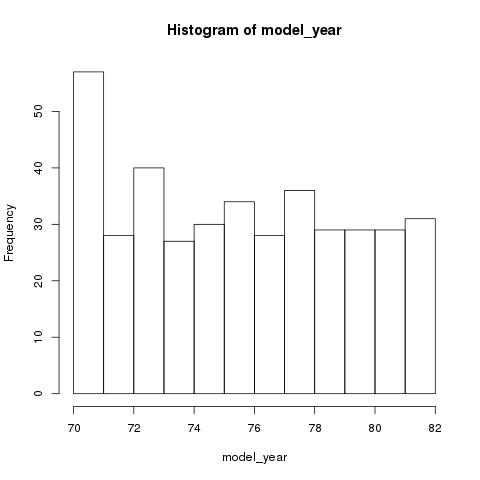
\includegraphics[scale=0.4]{model_year_histogram.jpg}
    \caption{lala}
    \label{fig:lala}
\end{figure}

Observando el gráfico es posible notar que entre los años 70 y 78 existe cierta irregularidad en la cantidad de modelos por
año, logrando la estabilidad desde el 78 en adelante. Las razones que puedan explicar esto son múltiples por ejemplo en aquellos años
no existía la renovación del vehículo por parte de cada dueño cada 1 o 2 años como ocurre hoy en día, además en los años 70 aún
era un mercado emergente que no permitía proyectar bien la demanda.

  \begin{minipage}{\linewidth}
      \centering
      \begin{minipage}{0.45\linewidth}
          \begin{figure}[H]
              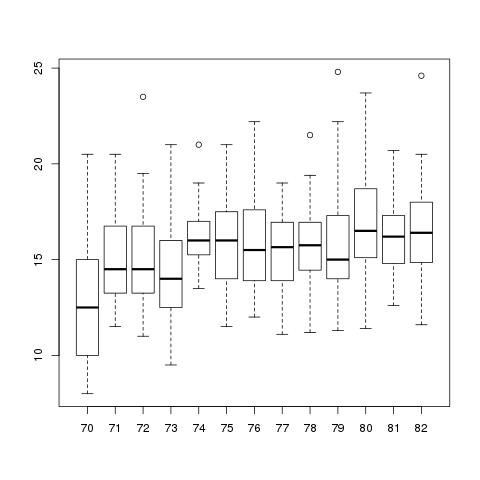
\includegraphics[width=\linewidth]{bp_acceleration_year.jpg}
              \caption{This is the first figure}
          \end{figure}
      \end{minipage}
      \hspace{0.05\linewidth}
      \begin{minipage}{0.45\linewidth}
          \begin{figure}[H]
              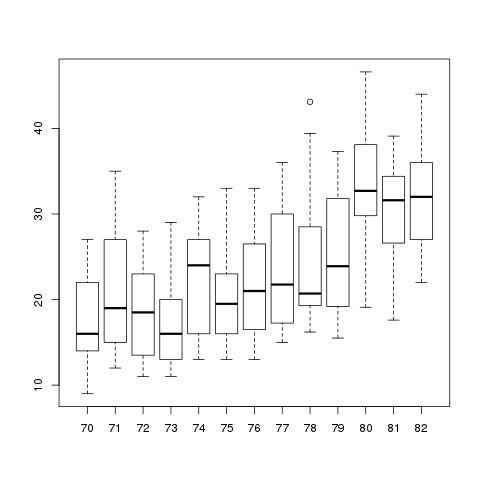
\includegraphics[width=\linewidth]{bp_mpg_year.jpg}
              \caption{This is the second figure}
          \end{figure}
      \end{minipage}
  \end{minipage}
  
    \begin{minipage}{\linewidth}
      \centering
      \begin{minipage}{0.45\linewidth}
          \begin{figure}[H]
              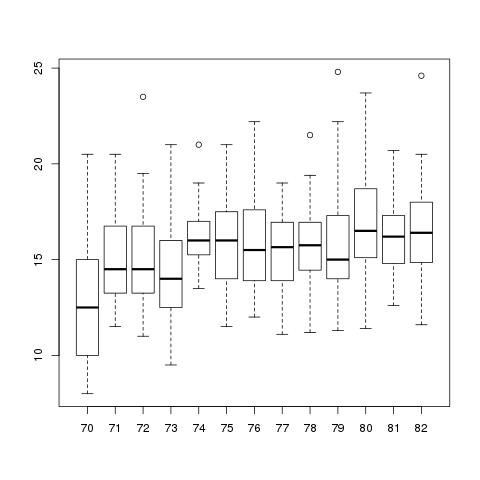
\includegraphics[width=\linewidth]{bp_acceleration_year.jpg}
              \caption{This is the first figure}
          \end{figure}
      \end{minipage}
      \hspace{0.05\linewidth}
      \begin{minipage}{0.45\linewidth}
          \begin{figure}[H]
              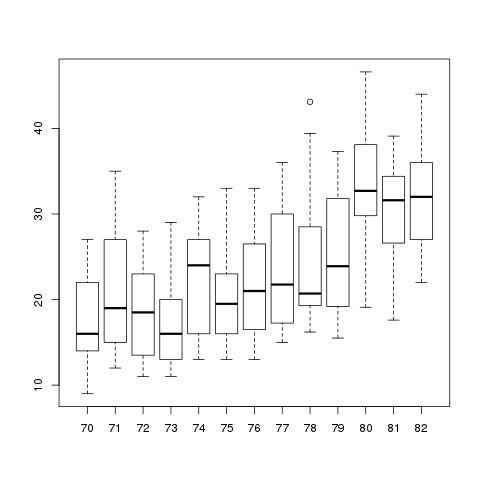
\includegraphics[width=\linewidth]{bp_mpg_year.jpg}
              \caption{This is the second figure}
          \end{figure}
      \end{minipage}
  \end{minipage}
  
  

\newpage

\subsection{Pregunta 3}

Intuitivamente se puede creer que una cilindrada alta implicaría un mayor número de cilindros en el motor,
pero eso no es suficiente para el análisis por lo que es necesario realizar boxplots
donde en un eje se encuentren la cilindrada y en otro la cantidad de cilindros con el fin
de partir el conjunto de cilindrada en grupos por cilindro ilustrados por los diagramas.
\begin{figure}[h!]
    \centering
    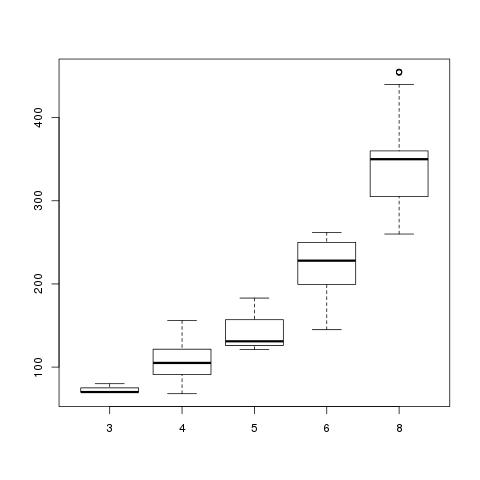
\includegraphics[scale=0.4]{boxplot_displacement_cylinders.jpg}
    \caption{lala}
    \label{fig:lala}
\end{figure}
A primera vista es posible observar que a medida que se aumentan los cilindros es posible
encontrar motores con mayor cilindradas. La mayoría de las cajas se encuentran acopladas solo por los bigotes lo que muestra
que existe una posible separación entre cada grupo de cilindros y la cilindrada posible pero es importante destacar que esto
no es una separación estricta sino que solamente la concentración de los datos entre cada grupo se encuentra distante donde los bigotes
permiten realizar la ``unión'' entre el conjunto de datos de cada boxplot lo cual indica que estos serían una cantidad mínima
de datos en relación a las cajas en si.
Otro elemento importante es que se puede observar una relación lineal con pendiente positiva entre los boxplot pero
la simple inspección no es suficiente por lo que se calculará la covarianza entre estas dos variables. La covarianza es
168.6232, al ser positiva implica una relación proporcional entre ambas variables por lo que las observaciones a partir
de los boxplot coinciden hasta cierto punto, pero la covarianza no nos entrega la intensidad de la relación por lo que se realiza
el cálculo de otra herramienta dispnonible hasta el momento, la cual es la correlación lineal, con un valor de 0.9507214
positiva y muy cercana a 1 implica una intensidad fuerte en la proporcionalidad entre los cilindros y la cilindrada de los modelos.
\begin{figure}[h!]
    \centering
    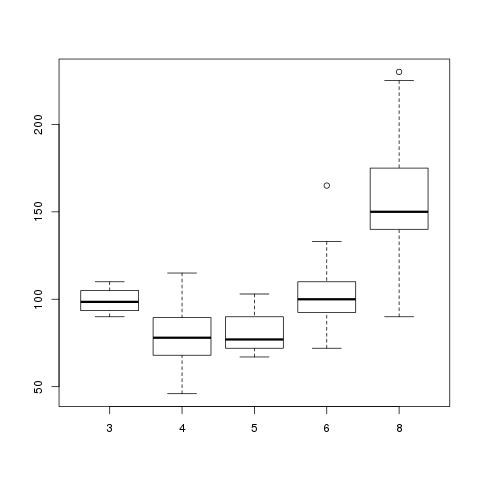
\includegraphics[scale=0.4]{boxplot_horsepower_cylinders.jpg}
    \caption{lala}
    \label{fig:lala}
\end{figure}
Nuevamente la mayor parte de los boxplot no estan desacoplados por lo que se puede percibir una relación entre ellos, a primera
vista se puede pensar que la relación será relativamente parecida a la anterior pero si se toma atención especial en los boxplot se pueden
descubrir elmentos que no dejarán desarrollar una hipótesis similar a la anterior.
A diferencia del caso anterior aquí se presenta una disminución en los valores de la potencia para las menores cantidades de cilindros.
Aparecen 2 datos atípicos, uno en la cantidad de cilindros 6 y otra en 8, donde ambos outliers son 
en valores muy altos en relación al resto que se encuentra
dentro de sus boxplot respectivos. Existen 2 boxplot que tienen bigotes ``largos'' mientras que el resto los tienen
 muy cortos en relación a su tamaño lo que da para pensar que existe poca dispersión en cada caso, 
 a esto hay que agregar que la mayoría de los boxplot tienen la concentración de los datos entre su primer cuartil y su mediana
 es decir que la mayor parte se encuentra en los valores menores dentro de su espectro de valores posibles, 
 además todas las medianas a excepción de la que corresponde a 8 cilindros, se encuentran en un valor cercano o menor a 100.
 El único que no lo cumple a su vez, resulta ser el boxplot que demuestra la mayor dispersión de los datos, nuevamente
 nos referimos a la cantidad de 8 cilindros, esto a priori permite imaginar que la dispersión de sus valores 
 no alcanza a hacer el correspondiente peso sobre el resto de los boxplot con fuertes concentraciones en 
 aceleraciones bajo los 100.
 Para acompañar la argumentación anterior se calcula la covarianza, esta es de $-2.370842$, al ser negativa entonces
 implica una relación inversamente proporcional 
 reafirmando gran parte de lo dicho anteriormente pero es necesario conocer su intensidad, por lo que se utilizará 
 la correlación lineal, siendo $-0.5054195$. Al encontrarse entre $-1$ y $0$ no es tan fácil afirmar que
 tan fuerte es la intensidad de la relación. Tal vez otro indicador que no busque ajustar mediante alguna recta los datos nos
 podría entregar una relación más precisa.
 


\newpage

\subsection{Pregunta 4}
\begin{figure}[h!]
    \centering
    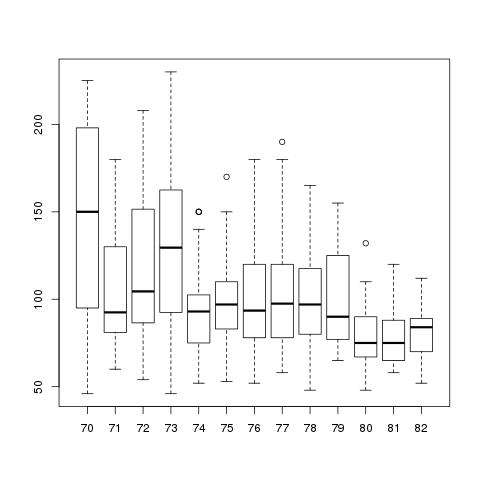
\includegraphics[scale=0.5]{boxplot_horsepower_model_year.jpg}
    \caption{lala}
    \label{fig:lala}
\end{figure}
\newpage
\subsection{Pregunta 5}

\begin{figure}[h!]
    \centering
    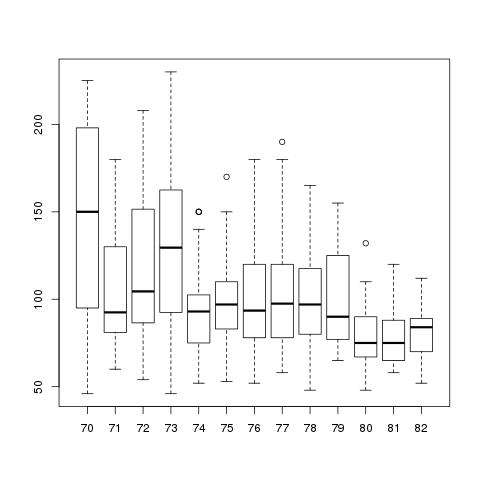
\includegraphics[scale=0.5]{boxplot_horsepower_model_year.jpg}
    \caption{lala}
    \label{fig:lala}
\end{figure}

\newpage
\subsection{Pregunta 6}

\begin{figure}[h!]
    \centering
    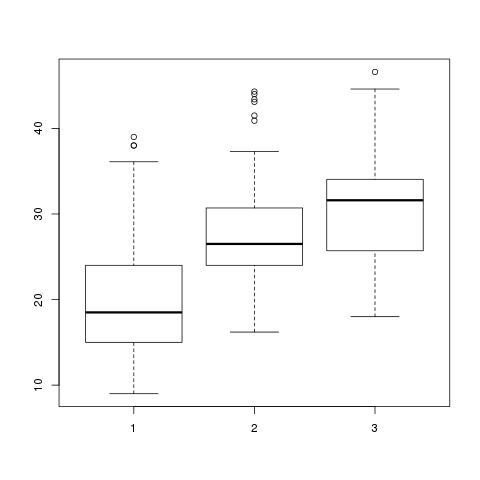
\includegraphics[scale=0.5]{boxplot_mpg_origin.jpg}
    \caption{lala}
    \label{fig:lala}
\end{figure}

\begin{figure}[h!]
    \centering
    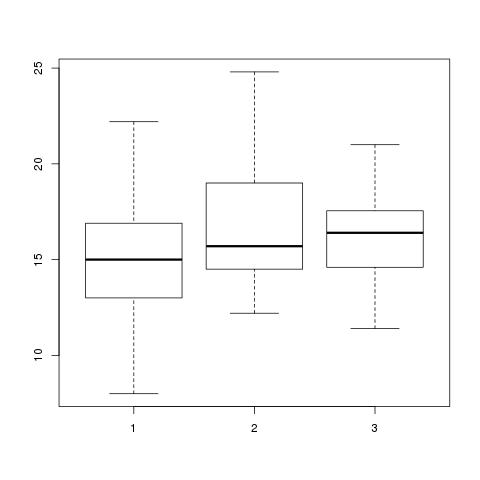
\includegraphics[scale=0.5]{boxplot_acceleration_origin.jpg}
    \caption{lala}
    \label{fig:lala}
\end{figure}

\begin{figure}[h!]
    \centering
    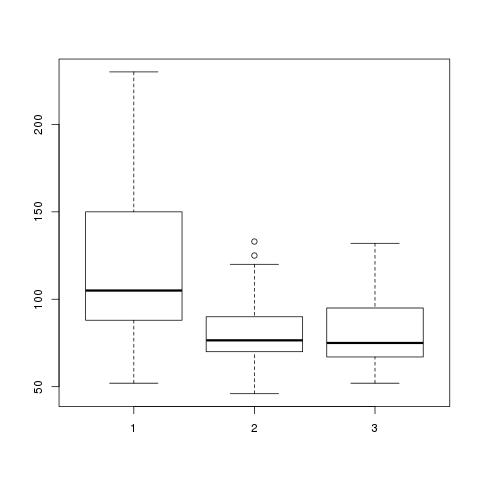
\includegraphics[scale=0.5]{boxplot_horsepower_origin.jpg}
    \caption{lala}
    \label{fig:lala}
\end{figure}


\subsection{Pregunta 7}

\subsection{Pregunta 8}


\section{Conclusiones}

\section{Anexos}


\bibliographystyle{alpha}
\bibliography{bibbase}

% referencias
[1] Nombre de la referencia, Autor.



\end{document}
